% TCBL Contrastive Learning Module Diagram
% Compile with XeLaTeX or LuaLaTeX

\documentclass[tikz,border=10pt]{standalone}
\usepackage{tikz}
\usetikzlibrary{shapes.geometric, arrows.meta, positioning, fit, backgrounds, calc, decorations.pathreplacing}

% Define colors
\definecolor{encblue}{RGB}{66,133,244}
\definecolor{projgreen}{RGB}{52,168,83}
\definecolor{contrastrange}{RGB}{255,152,0}
\definecolor{lossred}{RGB}{234,67,53}

\begin{document}
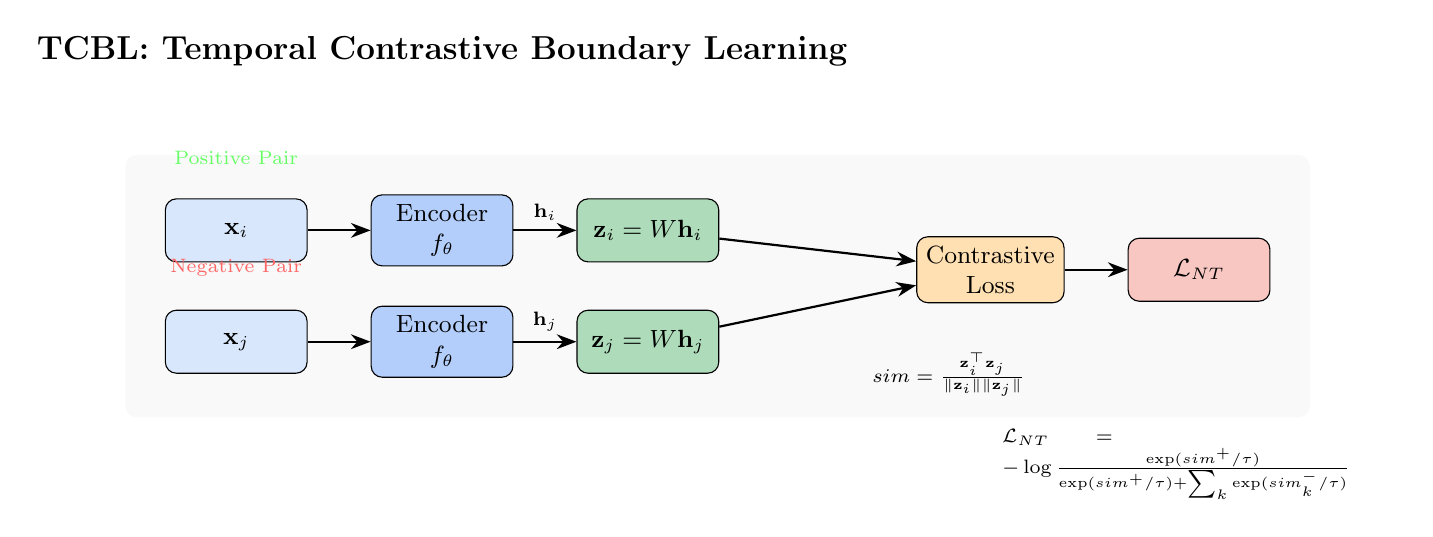
\begin{tikzpicture}[
    node distance=0.6cm and 0.8cm,
    block/.style={rectangle, draw, fill=#1, rounded corners, minimum height=0.8cm, minimum width=1.8cm, align=center, font=\small},
    block/.default=white,
    arrow/.style={-{Stealth[length=2.5mm]}, thick},
    label/.style={font=\scriptsize}
]

% Input windows
\node[block=encblue!20] (x1) {$\mathbf{x}_i$};
\node[block=encblue!20, below=of x1] (x2) {$\mathbf{x}_j$};

% Encoder
\node[block=encblue!40, right=of x1] (enc1) {Encoder\\$f_\theta$};
\node[block=encblue!40, right=of x2] (enc2) {Encoder\\$f_\theta$};

% Projections
\node[block=projgreen!40, right=of enc1] (z1) {$\mathbf{z}_i = W \mathbf{h}_i$};
\node[block=projgreen!40, right=of enc2] (z2) {$\mathbf{z}_j = W \mathbf{h}_j$};

% Contrastive loss
\node[block=contrastrange!30, right=2.5cm of z1, yshift=-0.5cm] (contrast) {Contrastive\\Loss};

% NT-Xent Loss
\node[block=lossred!30, right=of contrast] (loss) {$\mathcal{L}_{NT}$};

% Arrows
\draw[arrow] (x1) -- (enc1);
\draw[arrow] (x2) -- (enc2);
\draw[arrow] (enc1) -- node[above, label] {$\mathbf{h}_i$} (z1);
\draw[arrow] (enc2) -- node[above, label] {$\mathbf{h}_j$} (z2);
\draw[arrow] (z1) -- (contrast);
\draw[arrow] (z2) -- (contrast);
\draw[arrow] (contrast) -- (loss);

% Positive/Negative labels
\node[above=0.3cm of x1, font=\scriptsize, text=green!60] {Positive Pair};
\node[above=0.3cm of x2, font=\scriptsize, text=red!60] {Negative Pair};

% Similarity computation
\node[below=0.5cm of contrast, label, text width=3cm] {$sim = \frac{\mathbf{z}_i^\top \mathbf{z}_j}{\|\mathbf{z}_i\| \|\mathbf{z}_j\|}$};

% Title
\node[above=1.5cm of enc1, font=\large\bfseries] {TCBL: Temporal Contrastive Boundary Learning};

% Background
\begin{scope}[on background layer]
    \node[fit=(x1)(x2)(enc1)(enc2)(z1)(z2)(contrast)(loss), fill=gray!5, rounded corners, inner sep=0.5cm] {};
\end{scope}

% Formula
\node[below=1.5cm of loss, label, text width=5cm] {
    $\mathcal{L}_{NT} = -\log \frac{\exp(sim^+/\tau)}{\exp(sim^+/\tau) + \sum_k \exp(sim^-_k/\tau)}$
};

\end{tikzpicture}
\end{document}
